\renewcommand\thetable{\arabic{chapter}-\arabic{table}}
%\renewcommand\thefigure{\arabic{chapter}-\arabic{figure}}
\renewcommand{\theequation}{\arabic{chapter}-\arabic{equation}}
\chapter{相關研究}

作業系統指紋辨識的方法,可分為主動式作業系統指紋辨識(Active OS Fingerprinting )與被動式作業系統指紋辨識(Passive OS Fingerprinting )。主動式作業系統指紋辨識,主動對目標主機送出自製的探測封包,並根據回傳的反應做判斷依據,軟體工具Nmap與Xprobe2即屬於此類。Nmap主要控制TCP的參數值,做為探測用封包;Xprobe2則是著重於送出ICMP 封包,利用邏輯樹斷定作業系統的類型。被動式作業系統指紋辨識是監聽網路上目標主機的封包往來做為判斷的依據,P0f即屬於被動式,相對於主動式作業系統指紋辨識較不易被人察覺。不論是主動式或被動式的作業系統指紋辨識,皆利用TCP/IP堆疊進行辨識,包括封包存活時間(time to live, TTL)、Window Size、最大分割大小(Maximum Segment Size)、不分段標記(Don't Fragment flag)、Window Scale Option等,因為不同的作業系統的fingerprint有所不同,所以可做為判定作業系統的依據。如圖~\ref{fig:PHI}所示。


\begin{figure}[hbtp]
  \begin{center}
    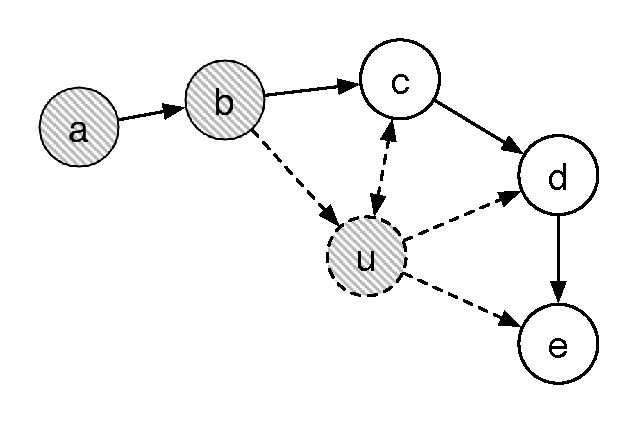
\includegraphics[width=1.0\textwidth]{figures/dyna_rm.eps}
    \caption{The diagram of ``prototypical PHI query''} 
    \label{fig:PHI}
  \end{center}
\end{figure}


網路發展興盛至今,小至個人,大至政府單位與各機關組織,都相當仰賴網路的使用,但許多人仍然對資安危機意識較低,針對資訊安全產品的投資也相對較少,加上對於資訊安全軟體工具缺乏有系統的整理,以致於未能有效運用。為此,本手冊蒐集整理相關開放源碼(Open Source)的資訊安全軟體工具,並透過專業人員實際操作演練,加以彙整並集結成冊,希冀透過本手冊的幫助,不僅能給予初學者對於資安工具軟體初步認識,也讓資訊從業人員在資訊安全工具上能有更多的選擇與應用。

資安開放源碼軟體的發展,往往會公開其發展技術及運用的原理,配合程式碼的開放,使得開放源碼軟體具有相當大的彈性,並根據個人使用情況所需,進行軟體的編修與整合,以求適應各種作業環境所需。使用開放源碼軟體所需負擔的金錢成本,遠低於商業付費軟體,可降低企業組織對資訊科技產品的部分支出,不需要過度仰賴軟體製造商的技術支援與更新,也能減少相對應的軟體開發時程。由於目前多數的資安開放源碼軟體的開發多為國外組織,因此較缺乏中文化介面,且部分軟體工具的使用,需要具備相當程度的專業知識,並非人人皆可輕易上手。本手冊擬透過中文化的工具介紹,減緩國內使用者入門的負擔。

由於現今網路環境日益複雜,遭受網路攻擊的事件層出不窮,網路安全越來越受到各界重視。網路掃描是網路安全的根本,也是攻擊者對目標主機進行攻擊的首要步驟,因此,了解網路掃描的攻擊與防禦,將有助於網路管理者提升網域的安全管理。此外,網路流量代表所有網路訊息的傳送,能提供管理者即時了解網路狀況,藉此檢視網路情況正常與否。本手冊將針對以上兩類的開放源碼軟體,逐一介紹其功能、安裝、操作與軟體評比,令讀者對相關的資訊軟體能有所了解,並進一步應用於資訊安全的監測與控管。以下即對網路掃描及流量監控兩大類軟體,進行整理與原理說明。
	
如表~\ref{tab:system}所示。 


\begin{table}[hbtp]
  \begin{center}
    \caption{The relation of aggregation overhead between different techniques}
    \label{tab:system}
    \begin{tabular}{|c|c c c|}
      \hline
       & Space usage & Communication & Query \\
       & of root aggregator & overhead & requirement \\
      \hline
      Traditional warehouse & $n$ & $O(n)$ & $O(n)$ \\
      \hline
      AM-FM sketch technique & $\log a$ & $O(\log n)$ &  $O(a\log n)$ \\
      \hline
      ``prototypical PHI query'' & $\log a$ & $O(\log n)$ & $O(\log n)$ \\
      \hline
      \end{tabular}
  \end{center}
\end{table}